\chapter{Graph Theory and Combinatorics}

Graph theory is concerned with the study of structures we call graphs as well as topics within combinatorics.
By \textit{graph}, we don't mean graphs in the $f(x)$ sense; rather, we are talking about nodes connected by edges.
Often times, we represent these graphs with a picture involving dots and lines, representative of vertices and edges, respectively.
Throughout our discussion, keep in mind that we cannot rely on a picture for a proof, but it is very helpful to see the pictures to get an understanding of what's happening.

\section{Introduction to Graphs}

The idea of a graph is relatively simple but requires some prior ideas from the study of set theory.
Recall that given a set $A$, we can create what is known as the power set of a, $\mathcal{P}(A)$, consisting of all subsets of $A$.
We can extend this idea a little further but considering subsets of the power set of a given set.

\begin{definition}{Power-$k$ Set}
    Let $A$ be a finite set of order $n$ and let $k\in\NN$.
    The power-$k$ set of $A$, $\mathcal{P}_{k}(A)$, is the set of all subsets of $A$ with cardinality $k$.
\end{definition}

We get some nice relationships between the power-$k$ set and the power set of $A$.
First, note that $\mathcal{P}_{k}(A)\subset\mathcal{P}(A)\ \forall k$; even if $k > n$, we still have a subset of $\mathcal{P}(A)$ since $\mathcal{P}_{k}(A)=\emptyset$ in that case.
The power set can be expressed as a union of power-$k$ sets:
\[
    \mathcal{P}(A) = \bigcup_{k=1}^{n}\mathcal{P}_{k}(A).
\]
There are various other properties that follow, but our main purpose of introducing the power-$k$ set is to assist us in our definition of a graph.

\begin{definition}{Graph}
    Let $V$ be a finite set and let $E\subset\mathcal{P}_{2}(V)$.
    The pair $(V,E)$ is called a graph, with the vertex set $V$ and the edge set $E$.
\end{definition}

This is our main definition to keep in mind throughout this entire chapter.
We may often see pictures of graphs drawn with dots and lines, but it is the pair of sets that truly defines the structure.
We can, and usually do, prefer to draw graphs from the provided sets in order to determine various properties.

\begin{example}{Let $V=\{a,b,c\}$ and $E=\{\{a,b\},\{b,c\}\}$. Draw a representation of this graph.}
    We ought to first determine whether or not $(V,E)$ actually is a graph.
    We require $E$ to have two main properties:

    \begin{enumerate}
        \item Every element of every set within $E$ is an element of $V$.
        \item $E\subset\mathcal{P}_{2}{V}$.
    \end{enumerate}

    Indeed, both these properties hold, so $(V,E)$ is a graph.
    We could draw infinitely many representations of $(V,E)$; here is one such.
    \begin{center}
        \begin{tikzpicture}[node distance=1cm]
            \node(a) {a};
    		\node(b) [below left of=a] {b};
    		\node(c) [below right of=a] {c};

    		\draw(a) -- (b);
    		\draw(b) -- (c);
        \end{tikzpicture}
    \end{center}
    The pairs within the $E$ represent the vertices which share an edge; the values within $V$ represent the vertices themselves.
\end{example}

One key fact to note is that the definition does not require the pairs within $E$ to be ordered; if they are ordered, then we have what is called a directed graph.
We also don't have any repeated edges (if we do, we have a multigraph), and no vertex can share an edge to itself (called a pseudograph)
We will look at directed graphs in depth later, but for now we will consider the non-directed case.

The next few pages will concern a whole slew of definitions.
The terminology here is not always standard, but it is what we will go with for the rest of our discussion on graphs.

\begin{definition}{Order}
    Suppose $G$ is a graph. Then the order of $G$ is $ord(G)=|V(G)|$.
\end{definition}
\begin{definition}{Size}
    Suppose $G$ is a graph. Then the size of $G$ is $size(G)=|E(G)|$.
\end{definition}

These terms are more for convenience. The next few are actually useful.

\begin{definition}{Degree}
    Let $v\in V(G)$. The degree of $v$ in $G$, $deg_{G}(v)$, is the number of edges incident with $v$.
    We often write $deg(v)$ if the context of the graph is obvious.
\end{definition}

The degree of a vertex tells us how many edges come out of the vertex.
As it so happens, we actually know how large this number can be: $ord(G) - 1$.
This makes sense intuitively; a vertex can have no duplicate edges and no edges to itself, so the max number of edges a given vertex can have is an edge to every other vertex in the graph.
If every vertex has this property, we call the graph \textit{complete}.

\begin{definition}{Complete}
    Let $G$ be a graph and let $n=ord(G)$. We call $G$ complete if $\forall\ v\in V(G),\ deg(v)=n-1$. Since these graphs are unique, we say $G=K_{n}$, meaning the complete graph on $n$ vertices.
\end{definition}

The concept of graph equality is something that we discuss further in a little bit.
For now, we are ready for our first theorem.

\begin{theorem}{}
    Suppose $G$ is a graph. Then
    \[
        \sum_{v\in V(G)}deg(v) = 2\ size(G).
    \]
\end{theorem}
\begin{proof}
    We can show this via induction. Suppose $size(G)=0$. Then $2\ size(G)=2\cdot0=0$.
    Since $size(G)=0$, $deg(v)=0\ \forall v\in V(G)$, so the sum over the degrees is also 0.
    Hence, we may assume for all graphs $H$ with $n$ edges,
    \[
        \sum_{v\in V(H)}deg_{H}(v) = 2n.
    \]
    Assume $G$ has $n+1$ edges. We must show
    \[
        \sum_{v\in V(G)}deg(v)=2(n+1).
    \]
    Let $H$ be a graph such that $V(H)=V(G)$ and $E(H)=E(G)\setminus ab$ for some $ab\in E(G)$. Then
    \[
        \sum_{v\in V(H)}deg_{H}(v)=2n\implies\sum_{v\in V(G)}deg_{H}(v)=2n.
    \]
    Since $ab\in E(G),\ \exists v_{1},v_{2}\in V(G)$ which are incident with $ab$.
    Hence $deg_{H}(v_{1})+1=deg_{G}(v_{1})$ and $deg_{H}(v_{2})+1=deg_{G}(v_{2})$.
    Note that for all other vertices in $v\in V(G)$, $deg_{H}(v)=deg_{G}(v)$.
    Then
    \[
        \sum_{v\in V(G)}deg_{H}(v)=-2+\sum_{v\in V(G)}deg_{G}(v).
    \]
    By the inductive hypothesis, we have
    \[
        2n=\left( \sum_{v\in V(G)}deg_{G}(v) \right) - 2\implies
        2(n+1)=\sum_{v\in V(G)}deg_{G}(v).
    \]
\end{proof}

Induction is a very common proof technique that we will encounter throughout or study of graphs; the strategy of creating a new graph with properties of our old graph is also a very useful technique.

\section{Walks, Paths, and Trails}

The topics covered in this section address the ways we can traverse graphs.
In our study, we have the freedom to move from any vertex to any other vertex as long as there is an edge between them.
The strategies we use to move around a graph form the theory of walks, paths, and trails.

\begin{definition}{Walk}
	Suppose $G$ is a graph. We say a finite sequence of vertices $v_{1},v_{2},\dots,v_{k}$ is a walk of length $k$ provided that $v_{i}v_{i+1}\in E(G)$ for all $1\leq i\leq k$. If $v_{1}=v_{k}$, then we say the walk is closed.
\end{definition}

In other words, a sequence of vertices is a walk if we can always move along a single edge to the next vertex in the sequence.
We have several ways to write walks; we can use set notation $\{a,b,c,d\}$ or simply write the vertices in the order they appear, $abcd$, if it is obvious to do so.

\begin{example}{}

	\begin{minipage}{0.3\textwidth}
		\begin{tikzpicture}[node distance=1cm]
			\node(a) {a};
			\node(b) [above right of=a] {b};
			\node(c) [below right of=b] {c};
			\node(d) [below of=c] {d};
			\node(e) [below left of=d] {e};

			\draw(a) -- (b);
			\draw(b) -- (c);
			\draw(c) -- (d);
			\draw(b) -- (d);
			\draw(d) -- (e);
		\end{tikzpicture}
	\end{minipage}
	\begin{minipage}[t]{0.65\textwidth}
        \vspace{-1.2cm}
		In this graph, $abde$ and $abcba$ form walks, but $ade$ does not since there is $ad\notin E(G)$.
        Note that we can repeat vertices if need be.
	\end{minipage}

\end{example}

Walks are simplistic in their construction since we can move anywhere in the graph where there is an edge.
The more interesting idea here is a walk where no vertices are repeated.

\begin{definition}{Path}
    Let $W$ be a walk in a graph $G$. If $W$ contains no repeated vertices, then we call $W$ a path. If we include the edge $v_{k}v_{1}$, provided that it exists, the we call the path closed, or a cycle.
\end{definition}

Paths concern vertices, but there is an analogous idea for edges.

\begin{definition}{Trail}
    If all edges in a walk are distinct, then it is called a trail.
\end{definition}

When talking about walks and paths, we say the length of the walk is the number of edges in the walk.
If the path is closed, then we count the missing edge in the path as part of the length.
With these definitions in mind, we now have enough to build our first theorem.

\begin{theorem}{}
    Let $G$ be a graph and let $A$ be a walk in $G$. If $A$ is not a trail, then $A$ is not a path.
\end{theorem}

We won't prove this here, but note that the contrapositive holds (and is a little more pleasing to read)

\begin{theorem}{}
    If $A$ is a path, then $A$ is a trail.
\end{theorem}

Again, we won't prove this, but it is important to keep in mind. The next theorem, however, is a little more worthwhile to prove.

\begin{theorem}{}
    Suppose $G$ is a graph and let $u,v\in V(G)$ be distinct. Then every $uv$ walk contains a $uv$ path.
\end{theorem}
\begin{proof}
    Let $A$ be a $uv$ walk, and assume $A$ has length 1. Hence, $u$ and $v$ are the only vertices in the walk, so $A$ is a path. Assume that all $uv$ walks of length $l$ contain a $uv$ path.
    We must show that for a $uv$ walk $A$ of length $l+1$ contains a $uv$ path.
    Since $A$ is a walk, we may name the vertices in $A$:
    \[
        A = v_{1}v_{2}\dots v_{k}
    \]
    with $u=v_{1}$ and $v=v_{k}$.
    If $A$ is a $uv$ path then we are done, so assume that $A$ is not a path.
    Then $\exists i\neq j \suchthat v_{i}=v_{j}$.
    Define $B$ to be a walk such that
    \[
        B = v_{1}v_{2}\dots v_{i}v_{j+1}v_{j+2}\dots v_{k}.
    \]
    We have removed at least one edge from $A$ to create $B$, so the length of $B$ is less than or equal to $l$.
    By the inductive hypothesis, we have that $B$ contains a $uv$ path $C$.
    Hence if $C$ is contained in $B$ and $B$ is contained in $A$, then $C$ is contained in $A$, so $A$ contains a $uv$ path.
\end{proof}

This is a very important result since it allows us to find a $uv$ path in any $uv$ walk.

\section{Types of Graphs}

A typical graph probably does not have any special characteristics that set that graph apart from others.
There are, however, a whole slew of graphs that are recognized separately from a typical graph.
Among these are complete graphs and bipartite graphs, which we will examine here.

\subsection*{Complete Graphs}

To grasp the concept of a complete graph, we must first understand the idea of connectedness.
We will, as is common in graph theory, begin with a definition.

\begin{definition}{Connected}
	A graph $G$ is called connected if for every pair of vertices $u,v\in V(G)$, there is a $uv$ walk in $G$.
	$G$ is called disconnected if it is not connected.
\end{definition}

In other words, we can get from any vertex to any other vertex in the graph no matter what.
It is especially important to realize that pictures can deceive us here, as the next example will show.

\begin{example}{Determine if the following graph is connected}
	\begin{center}
		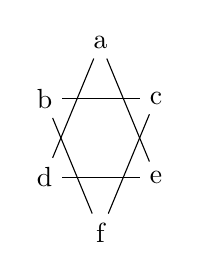
\begin{tikzpicture}[node distance=1cm]
			\node(a) {a};
			\node(b) [below left of=a] {b};
			\node(c) [below right of=a] {c};
			\node(d) [below of=b] {d};
			\node(e) [below of=c] {e};
			\node(f) [below right of=d] {f};

			\draw(a) -- (d);
			\draw(d) -- (e);
			\draw(e) -- (a);
			\draw(b) -- (f);
			\draw(f) -- (c);
			\draw(b) -- (c);
		\end{tikzpicture}
	\end{center}

	As it turns out, this graph is not connected, since there is no $ab$ path, even though the two cycles are drawn on top of each other.
\end{example}

In the above example, we can see two cycles, $adea$ and $bcfb$.
These two cycles are completely disjoint from each other; we cannot start on one and get to the other.
Hence, the two cycles actually form smaller graphs themselves. We call them \textit{subgraphs}

\begin{definition}{Subgraph}
	Suppose $G$ is a graph, and let $H$ be a graph such that $V(H)\subset V(G)$ and $E(H)\subset E(G)$.
	Then $H$ is a subgraph of $G$, denoted by $H\leq G$.
\end{definition}

In our case, we actually have two disconnected subgraphs who together from $G$.
If this is the case, we can take the concept of subgraphs a step further.

\begin{definition}{Connected Component}
	Suppose $G$ is a graph, and let $H$ be a graph such that $H\leq G$. Then $H$ is called a connected component if
	\begin{enumerate}
		\item $H$ is connected
		\item $v\in V(H)$ and $u\in V(G)\setminus V(H) \implies$ there is no $uv$ path in $G$.
	\end{enumerate}
\end{definition}

This is exciting, since we can now say $adea$ and $bcfb$ form connected components of $G$.
Not all graphs will contain connected components, however; if this is the case, we might be interested in trying to create connected components by removing either a vertex or an edge from the graph.
If we can accomplish this, then we call the removed vertices or edges by special names.

\begin{definition}{Cut Vertex}
	Let $G$ be a graph with $v\in V(G)$. Then $v$ is called a cut vertex of $G$ if the graph formed by removing $v$, $G-v$, has more connected components that $G$.
\end{definition}

We need to be a little cautious when we say \textit{remove $v$}; removing a vertex requires us to remove all the edges incident with that vertex as well.

\begin{example}{Determine the cut vertices of the following graph.}
	\begin{center}
		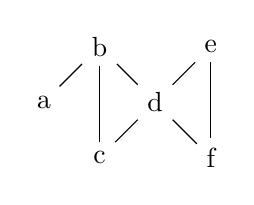
\begin{tikzpicture}[node distance=1cm]
			\node(a) {a};
			\node(b) [above right of=a] {b};
			\node(c) [below right of=a] {c};
			\node(d) [above right of=c] {d};
			\node(e) [above right of=d] {e};
			\node(f) [below right of=d] {f};

			\draw(a) -- (b);
			\draw(b) -- (c);
			\draw(b) -- (d);
			\draw(c) -- (d);
			\draw(d) -- (e);
			\draw(d) -- (f);
			\draw(e) -- (f);
		\end{tikzpicture}
	\end{center}

	We need to identify vertices that create connected components upon their removal. The vertex $d$ does the job here, since $G-d$ looks like

	\begin{center}
		\begin{tikzpicture}[node distance=1cm]
			\node(a) {a};
			\node(b) [above right of=a] {b};
			\node(c) [below right of=a] {c};
			\node(d) [above right of=c] {};
			\node(e) [above right of=d] {e};
			\node(f) [below right of=d] {f};

			\draw(a) -- (b);
			\draw(b) -- (c);
			\draw(e) -- (f);
		\end{tikzpicture}
	\end{center}
	where one connected component is given by the vertices $abc$ and the other by the vertices $ef$.
	There is another vertex that works here: $b$. Note that a single vertex is connected by definition, and $G-b$ looks like
	\begin{center}
		\begin{tikzpicture}[node distance=1cm]
			\node(a) {a};
			\node(b) [above right of=a] {};
			\node(c) [below right of=a] {c};
			\node(d) [above right of=c] {d};
			\node(e) [above right of=d] {e};
			\node(f) [below right of=d] {f};

			\draw(c) -- (d);
			\draw(d) -- (e);
			\draw(d) -- (f);
			\draw(e) -- (f);
		\end{tikzpicture}
	\end{center}

	where $a$ is one connected component and $c,d,e,$ and $f$ are in the other connected component.
\end{example}

Similarly, we have a definition for edges that accomplish this task.
Removal of edges is simpler than vertices, however, since we need not worry about the vertices incident with the edge.

\begin{definition}{Bridge}
	Let $G$ be a graph with $e\in E(G)$. Then $e$ is called a bridge of $G$ if the graph formed by removing $e$, $G-e$, contains more connected components than $G$.
\end{definition}

Vertices seem to be the more interesting object to remove from a graph, so we will focus on them a little more than edges.
We have a special name for the set of vertices that are cut verticies.

\begin{definition}{Cut Set}
	Let $G$ be a graph and let $S\subset V(G)$. $S$ is called a cut set of $G$ if the graph with vertex set $V(G)\setminus S$ is disconnected.
\end{definition}

In other words, if we remove all the cut vertices from a graph, we expect that graph to be disconnected.
Indeed, this makes intuitive sense, since any graph with more than one connected component is disconnected, and cut vertices create connected components.
With the notion of cut set, we can finally introduce completeness of graphs.

\begin{definition}{Complete}
	Let $G$ be a graph. $G$ is called complete if and only if $G$ has no cut sets.
	We denote a complete graph by $K_{n}$ where $n=ord(G)$.
\end{definition}

A complete graph consists of $n$ vertices that have every edge possible; hence removing one of the vertices isn't a problem since every other vertex is still connected to any other vertex in the graph.

\begin{example}{}
	The following are examples of complete graphs.
	\begin{center}
		\begin{tabular}{c c c}
			\begin{tikzpicture}[node distance=1cm]
                \node(a) {a};
                \node(b) [left of=a] {b};

                \draw(a) -- (b);
			\end{tikzpicture} &
			\begin{tikzpicture}[node distance=1cm]
                \node(a) {a};
                \node(b) [below right of=a] {b};
                \node(c) [above right of=b] {c};

                \draw(a) -- (b);
                \draw(b) -- (c);
                \draw(c) -- (a);
			\end{tikzpicture} &
			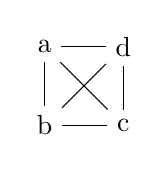
\begin{tikzpicture}[node distance=1cm]
                \node(a) {a};
                \node(b) [below of=a] {b};
                \node(c) [right of=b] {c};
                \node(d) [above of=c] {d};

                \draw(a) -- (b);
                \draw(a) -- (c);
                \draw(a) -- (d);
                \draw(b) -- (c);
                \draw(b) -- (d);
                \draw(c) -- (d);
			\end{tikzpicture}\\
            $K_{2}$ & $K_{3}$ & $K_{4}$
		\end{tabular}
	\end{center}
\end{example}

\subsection*{Bipartite Graphs}

The next type of graph we will study is called a bipartite graph.
Bipartite graphs are unique in that they can be partitioned into two sets that contain disconnected vertices.

\begin{definition}{Bipartite}
    Let $G$ be a graph and let $W\subset V(G)$. $G$ is called bipartite if for every edge in $uv\in E(G)$, either $u\in W$ and $v\in V(G)\setminus W$, or $u\in V(G)\setminus W$ and $v\in W$.
\end{definition}

